% =========================================================	
\newpage
\section{Interpolation}
% =========================================================	

\defi{
	\n
	Interpolation bedeutet im Grunde, eine unbekannte Funktion aufgrund von gegebenen Teilinformationen zu erraten bzw. mathematisch würde man natürlich von annähern sprechen.
	\n
	%		Wenn man beispielsweise weiß, dass eine Funktion zwischen zwei bestimmte Punkte geht aber sonst nichts, wäre eine bestmögliche Annäherung eine Gerade, nämlich solche, die beide Punkte miteinander verbindet.
	Formal: Finde zu $n$ Stützstellen ($x_i, f(x_i)$) einer unbekannten Funktion $f(x)$ eine Funktion $p(x)$, mit 
	\begin{align*} 
		p(x_i) = f(x_i) \; \forall x_i \quad (i = 0, \dots, n-1)
	\end{align*}
	Das bedeutet nur, dass eine Interpolation von Punkten $p(x)$ einer Funktion $f(x)$ durch alle Stützpunkte "hindurchgeht". Da wir ja sonst von keinerlei Informationen über $f(x)$ ausgehen ist das natürlich der beste Weg, weil zumindest diese Punkte stimmen und der Rest approximiert wird.
}
	\lbreak
	% ------------------------------------	
	\subsection{Polynominterpolation}
	% ------------------------------------	
	\sbreak
	\defi{
		\n 
		Jetzt soll es erst einmal nur um die Polynominterpolation gehen, also eine Annäherung einer unbekannten Funktion durch eine Polynomfunktion. Andere Methoden wären mit trigonometrischen Funktionen (siehe \refChapter{chap:Frequenzanalyse}) und linearer Interpolation (siehe \refChapter{chap:linearInterpolation}).
		\n 
		Unsere Ergebnisse sind, wie der Name schon impliziert, immer Polynome und damit im Gegensatz zur linearen Interpolation stetig und beliebig häufig stetig differenzierbar.
		\n
		Wiederholung Polynom $k$'ten Grades: 
		\begin{align*}
			c_k x^k + c_{k-1}x^{k-1} + \dots + c_1x^1 + c_0
		\end{align*}
		Wir können das Problem leicht in ein LGS übersetzen, indem wir einfach ein allgemeines Polynom $(n-1)$'ten Grades aufstellen und unsere Stützpunkte einsetzen. Wir definieren mit $y_i = f(x_i)$ die $y$ Koordinaten der Stützpunkte (auch Stützwerte genannt).
		\begin{align*}
			\begin{bmatrix}
				x_0^{0} & x_0^{1} & \dots & x_0^{n-1}\\
				x_1^{0} & x_1^{1} & \dots & x_1^{n-1}\\
				\vdots & \vdots & \ddots & \vdots \\
				x_{n-1}^{0} & x_{n-1}^{1} & \dots & x_{n-1}^{n-1}
			\end{bmatrix} &\cdot
			\nvector{
				c_0 \\ \vdots \\ c_{n-2} \\ c_{n-1}
			} = 
			\nvector{
				y_0 \\ \vdots \\ y_{n-2} \\ y_{n-1}
			}
		\end{align*}
		Die Lösungsfunktion (Interpolationsfunktion genannt) erhalten wir, indem wir die ausgerechneten Koeffizienten $c_0$ bis $c_{n-1}$ in unsere allgemeine Polynomfunktion $(n-1)$'ten Grades einsetzen.
		Also erhalten wir für $n$ Stützstellen immer ein Polynom $(n-1)$'ten Grades!
	}

	\lbreak
	\subsubsection{Basisfunktionen} \label{chap:basisfunktionen}
	
	\defi{
		\n 
		Das Kalkulieren mit Basisfunktionen (und damit mithilfe eines LGS) liegt in $\bigO(n^3)$, für die Auswertung der entstehenden Funktion $\bigO(n)$.
		Unter den Standard Polynom Basisfunktionen versteht man
		\begin{align*}
			g_0(x) &= 1 	&& g_1(x) = x\\
			g_2(x) &= x^2 	&& g_3(x) = x^3 \\
			\vdots
		\end{align*}
	}
	
	\sbreak
	\methode{
		\n 
		Unser Problem können wir als LGS mit allgemeinen Basisfunktionen darstellen. Wir haben immer genauso-viele Gleichungen ($n$ Stützstellen) wie wir Unbekannte ausrechnen möchten, da der Grad des resultierenden Polynoms mit steigendem $n$ linear korreliert.
		\n
		Umgerechnet mit beliebigen Basisfunktionen $g_0$ bis $g_{n-1}$:
		\begin{align}
			\begin{bmatrix}
				g_0(x_0) & g_1(x_0) & \dots & g_{n-1}(x_0)\\
				g_0(x_1) & \ddots & \ddots & g_{n-1}(x_1)\\
				\vdots & \ddots & \ddots & \vdots \\
				g_0(x_{n-1}) & \dots & \dots & g_{n-1}(x_{n-1})
			\end{bmatrix} \cdot
			\nvector{
				c_0 \\ \vdots \\ c_{n-2} \\ c_{n-1}
			} =
			\nvector{
				y_0 \\ \vdots \\ y_{n-2} \\ y_{n-1}
			}
		\end{align}
		Die Interpolationfunktion und damit Lösung des Problems entspricht dann:
		\begin{align} 
			p(x) = c_0 \cdot g_0(x) + c_1 \cdot g_1(x) + \dots + c_{n-1} \cdot g_{n-1}(x) 
		\end{align}
	}
	
	\newpage
	\bsp{ \n
		Eine unbekannte Funktion $f$ durchläuft folgende Punkte:
		\begin{align*}
			f(1) = 0 \aae f(2) = 2
		\end{align*}
		Wir haben also ein $n = 2$ und berechnen ein Polynom $(n - 1) = 1$'ten Grades. Wir sollen das Interpolationspolynom mithilfe der Standard Polynom Basisfunktionen aufstellen und damit den Funktionswert an der Stelle $1.5$ abschätzen. Bis Grad $1$ sind die Basisfunktionen also $g_0(x) = 1$ und $g_1(x) = x$.
		\\
		Stellen wir unseres LGS auf:
		\begin{align*}
			\begin{bmatrix}
				1 & 1\\
				1 & 2
			\end{bmatrix} \cdot 
			\nvector{
				c_0\\ c_1
			} = 
			\nvector{
				0 \\ 2
			}
		\end{align*}
		Mit Gauß aufgelöst erhalten wir 
		\begin{align*}
			c = (-2, 2)\trans
		\end{align*}
		Das wiederum (mit den Basisfunktionen) ergibt die Funktion
		\begin{align*}
			p(x) &= c_0 \cdot g_0(x) + c_1 \cdot g_1(x) \\
			p(x) &= c_0 \cdot 1 + c_1 \cdot x \\
			p(x) &= (-2) + 2 \cdot x
		\end{align*}
		Jetzt noch einsetzen:
		\begin{align*}
			p(1.5) = -2 + 3 = 1
		\end{align*}
		%
		\begin{figure}[H]
			\centering
			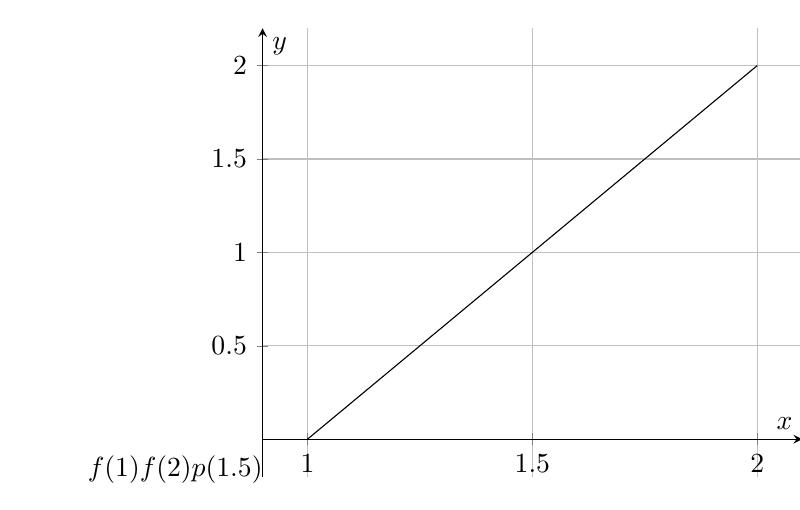
\begin{tikzpicture}
				\begin{axis}[
					axis lines=middle,
					xlabel=$x$,
					ylabel=$y$,
					enlargelimits,
					grid=major,
					legend pos=outer north east,
					%ymin=-0.3,
					%xmax=5.8,
					%xticklabels={,,},
					xtick={0, 1, 1.5, 2, 2.5},
					%yticklabels={,,},
					]
					\addplot[domain=1:2] {2*x - 2} node[left]{};
					\tikzPointUp{$f(1)$}{1,0}
					\tikzPointDown{$f(2)$}{2,2}
					\tikzPointDR{$p(1.5)$}{1.5,1}
					\legend{$p(x)$}
				\end{axis}
			\end{tikzpicture}
			\caption{Das Beispiel grafisch veranschaulicht.}
		\end{figure}
	}
	
	\sbreak
	\subsubsection{Lagrange-Basis} \label{sec:lagrange_basis}
	
	\sbreak
	\defi{ 
		\n
		Die Lagrange-Basis soll eine Möglichkeit sein, "schlaue" Basisfunktionen zu erstellen. \\
		Folgendermaßen wird sie berechnet: 
		\begin{align} 
	 		L_j = \prod_{i = 0; i \neq j}^{n-1} \frac{x - x_i}{x_j - x_i} 
	 	\end{align}
		Wenn man die $L_j$ nun als Basisfunktionen $g_0, \dots, g_{n-1}$ verwendet und das LGS lösen will, stellt man fest, dass die linke Matrix immer der Einheitsmatrix $\unitM$ entspricht und das Lösen des LGS trivial macht. Das liegt daran, dass die "schlauen" Basisfunktionen eben nur an der Stelle der jeweiligen Stützstelle $1$ beträgt und an allen anderen $0$.
		Ohne das LGS zu berechnen entsteht also die Interpolationspolynomfunktion 
		\begin{align} 
	 		p(x) = \sum_{j = 0}^{n-1}y_j \cdot L_j(x) 
	 	\end{align}
		Hier sehen wir, dass das Aufstellen der Funktion faktisch gar nichts kostet (bzw. $\bigO(n)$), das Auswerten der Interpolationsfunktion jedoch $\bigO(n^2)$!
	}
	
	\sbreak
	\bsp{
		\n
		Wir haben die Punktemenge von Stützstellen gegeben mit:
		\begin{align*}
			P: 
			\begin{Bmatrix}
				(0,1), (1,4), (3, -2)
			\end{Bmatrix}
		\end{align*}
		Wir möchten mithilfe von Lagrange-Basisfunktionen das Interpolationspolynom aufstellen:
		\begin{align*}
			L_0 &= \frac{(x - 1)(x - 3)}{(0 - 1)(0 - 3)} = \frac{(x - 1)(x - 3)}{3}\\
			L_1 &= \frac{(x - 0)(x - 3)}{(1 - 0)(1 - 3)} = \frac{x \cdot (x - 3)}{-2}\\
			L_2 &= \frac{(x - 0)(x - 1)}{(3 - 0)(3 - 1)} = \frac{x \cdot (x - 1)}{6}
		\end{align*}
		Jetzt noch die Interpolationsfunktion ausrechnen:
		\begin{align*}
			p(x) &= 1 \cdot L_0 + 4 \cdot L_1 -2 \cdot L_2 \\
				&= 1 \cdot \frac{(x - 1)(x - 3)}{3} + 4 \cdot \frac{x \cdot (x - 3)}{-2} - 2 \cdot \frac{x \cdot (x - 1)}{6} \\
				&= 1 + 5 \cdot x - 2 \cdot x^2
		\end{align*}
		\n 
		\begin{figure}[H]
			\centering
				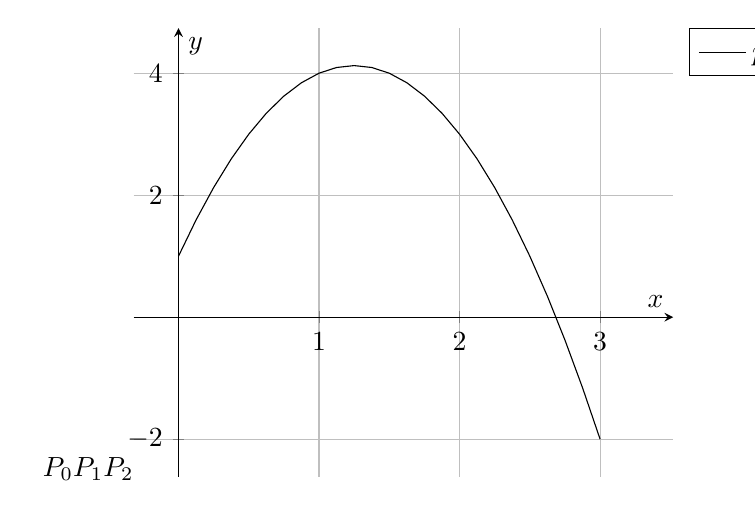
\begin{tikzpicture}
					\begin{axis}[
						axis lines=middle,
						xlabel=$x$,
						ylabel=$y$,
						enlargelimits,
						legend pos=outer north east,
						grid=major,
						xmax=3.2,
						%ymin=-0.3,
						%xmax=5.8,
						%xticklabels={,,},
						%yticklabels={,,},
						]
						\addplot[domain=0:3] {1 + 5*x^1 - 2*x^2} node[left]{};
						\tikzPointRight{$P_0$}{0,1}
						\tikzPointDR{$P_1$}{1,4}
						\tikzPointUR{$P_2$}{3,-2}
						\legend{$p(x)$}
					\end{axis}
				\end{tikzpicture}
			\caption{Das Beispiel grafisch veranschaulicht.}
		\end{figure}
	}

	\sbreak
	\wichtig{ \label{chap:polynomInterpolationEindeutigkeit}
		\n
		Ein Interpolationspolynom ist stets \fat{eindeutig}! Egal ob man die Standard Polynom Basisfunktionen, die Lagrange Basis oder so verwendet kommt zu einem Problem immer dasselbe Polynom raus. Auf Genauigkeit brauchen wir also keinen dieser Algorithmen untersuchen, jedoch aber die Anzahl an darstellbaren Polynomgraden (im Moment $n-1$ für $n$ Stützstellen). 
	}


	\newpage
% =========================================================	
	\subsubsection{Interpolation nach Newton} \label{chap:newtoninterpolation}
% =========================================================	
	
	\sbreak
	\defi{
		\n
		Die Interpolation nach Newton ist ein effizienterer Algorithmus, ein Interpolationspolynom analytisch auszurechnen, denn das Verfahren braucht für das Berechnen der Koeffizienten nur $\bigO(n^2)$ und das Auswerten der Funktion auch nur $\bigO(n)$.
	}

	\sbreak
	\methode{
		\n
		Wir definieren:
		\begin{align}
			c_{i,0} &= f(x_i) = y_i \\
			c_{i,k} &= \frac{c_{i+1,k-1} - c_{i,k-1}}{x_{i+k} - x_i}
		\end{align}
		Informeller ist folgendes:
		\begin{align} 
 			[\text{neu}]c = \frac{f\uleftDown - f\uleft}{x\uleftDiagonal - x\uleft} 
 		\end{align}
		Dabei sind die Richtungen immer in Relation zu der Stelle des zu ausrechnenden Wertes in der Tabelle angegeben. "ganzLinksUnten" meint, dass man in der Tabelle soweit nach ganz links unten zieht, bis man mit dem nächsten "Links-Unten-Move" nicht mehr in der rechten Seite der Tabelle wäre. Von dort aus nimmt man den x-Wert ganz links in derselben Zeile.
		\begin{table}[H]
			\label{table:newton}
			\centering
			\begin{tabular}{cc|cccc}
				\toprule
				$x_i$  & $i \setminus k$ & 0 & 1 & 2 & \dots \\ \midrule
				$x_0$ & $0$ & $c_{0,0}$ & $c_{0,1}$ & $c_{0,2}$ & \dots \\
				$x_1$ & $1$ & $c_{1,0}$ & $c_{1,1}$ & \mddots & \\
				$x_2$ & $2$ & $c_{2,0}$  & \mddots & & \\
				\vdots & & \mddots & & & \\
			\end{tabular}
			\caption{Tabelle zum Ausrechnen}
		\end{table}
		\noindent Wenn wir das fertig aufgestellt haben, können wir direkt alle Koeffizienten ablesen:
		\begin{align} 
			p(x) = c_{0,0} + c_{0,1} \cdot (x-x_0) + \dots + c_{0,n-1} \cdot \prod_{i=0}^{n-2}(x-x_i)
		\end{align}
		Unsere Koeffizienten sind also einfach die Werte der ersten Zeile der Tabelle.
	}

	\newpage
	\bsp{ \n 
		Wir haben:
		\begin{table}[H]
			\centering
			\begin{tabular}{cc|cccc}
				\toprule
				$x_i$  & $i \setminus k$ & 0 & 1 & 2 \\ \midrule
				$0$ & $0$ & $0$ & $c_{0,1}$ & $c_{0,2}$ \\
				$2$ & $1$ & $4$ & $c_{1,1}$ & \\
				$3$ & $2$ & $9$ & &
			\end{tabular}
		\end{table}%
		\begin{align*} 
 			c_{0,1} &= \frac{4 - 0}{2 - 0} = 2 \\
 			c_{1,1} &= \frac{9 - 4}{3 - 2} = 5 \\
			c_{0,2} &= \frac{5 - 2}{3 - 0} = 1 
		\end{align*}
		\begin{table}[H]
			\centering
			\begin{tabular}{cc|cccc}
				\toprule
				$x_i$  & $i \setminus k$ & 0 & 1 & 2 \\ \midrule
				$0$ & $0$ & $0$ & $2$ & $1$ \\
				$2$ & $1$ & $4$ & $5$ & \\
				$3$ & $2$ & $9$ & & \\
			\end{tabular}
		\end{table}
		Also kommt als Interpolationsfunktion folgendes heraus:
		\begin{align*} 
	 		p(x) &= c_{0,0} + c_{0,1} \cdot (x - x_0) + c_{0,2} \cdot (x - x_0)(x-x_1) \\
	 		&= 0 + 2 \cdot (x - 0) + 1 \cdot (x - 0)(x - 2) \\
	 		&= 0 + 2x + 1 \cdot x^2 - 2x \\
	 		&= x^2
	 	\end{align*}
		Würden wir hier die Punkte oben betrachten, sehen wir schon, dass es auf $x^2$ hinauslaufen wird.
	}

	\sbreak
	\defi{
		\n 
		Es ist vielleicht schon zu erkennen, aber wenn jetzt noch ein neuer Stützpunkt hinzugefügt werden soll, kann man diesen in der Tabelle einfach darunter schreiben und den neuen Koeffizienten relativ schnell ausrechnen. Dann muss nur noch das Ergebnis angepasst werden, indem ein weiteres Summenglied hinzugefügt wird und wir sind schon fertig. Das ist ein \fat{großer Vorteil} dieses Verfahrens.
	}

	\newpage
	\bsp{
		\n 
		Wir erweitern letztes Beispiel um einen weiteren Stützpunkt, und zwar mit $(-2, 4)$.
		\begin{table}[H]
			\centering
			\begin{tabular}{cc|ccccc}
				\toprule
				$x_i$  & $i \setminus k$ & 0 & 1 & 2 & 3
				\\ \midrule
				$0$ & $0$ & $0$ & $2$ & $1$ & $c_{0,3} = ?$\\
				$2$ & $1$ & $4$ & $5$ & $?$ &\\
				$3$ & $2$ & $9$ & $?$ & &\\
				$-2$ & $3$ & $4$ & & &
			\end{tabular}
		\end{table}
		\noindent Wir müssen die mit Fragezeichen markieren Stellen noch ausrechnen, um auf den neuen Koeffizienten $c_{0,3}$ schließen zu können.
		\begin{align*} 
			c_{2,1} &= \frac{4 - 9}{-2 - 3} = 1 \\
			c_{1,2} &= \frac{1 - 5}{-2 - 2} = 1 \\
			c_{0,3} &= \frac{1 - 1}{-2 - 0} = 0 = c_3
		\end{align*}
		Insgesamt sieht die Tabelle also folgendermaßen aus:
		\begin{table}[H]
			\centering
			\begin{tabular}{cc|ccccc}
				\toprule
				$x_i$  & $i \setminus k$ & 0 & 1 & 2 & 3
				\\ \midrule
				$0$ & $0$ & $0$ & $2$ & $1$ & $0$\\
				$2$ & $1$ & $4$ & $5$ & $1$ &\\
				$3$ & $2$ & $9$ & $1$ & &\\
				$-2$ & $3$ & $4$ & & &
			\end{tabular}
		\end{table}
		\noindent Jetzt noch die Interpolationsfunktion ausrechnen:
		\begin{align*} 
			p(x) &= c_{0,0} + c_{0,1} \cdot (x - x_0) + c_{0,2} \cdot (x - x_0)(x - x_1) + c_{0,3} \cdot (x - x_0)(x - x_1)(x - x_2)\\
			&= 0 + 2 \cdot (x - 0) + 1 \cdot (x - 0)(x - 2) + 0\\
			&= 0 + 2x + 1 \cdot x^2 - 2x \\
			&= x^2
		\end{align*}
		Das Ergebnis ist logisch, da der neue Punkt $(-2, 4)$ auch auf der Funktion $x^2$ liegt. Die Hinzunahme dieses Stützpunktes dürfte unser Ergebnis gar nicht abändern! Das können wir außerdem daher ablesen, dass der neu berechnete Koeffizient $0$ ist und damit keinen Einfluss auf die Ergebnisfunktion hat.
	}
	
	\newpage
% =========================================================	
	\subsubsection{Aitken-Neville}
% =========================================================	
	
	\defi{\n
		Dieses Verfahren dient dazu, ein Interpolationspolynom \fat{direkt an einer Stelle x auszuwerten}, obwohl wir das Polynom selbst nie ausgerechnet haben. Aitken-Neville rechnet das Polynom auch nicht direkt aus.
		\n
		Das machen wir, indem wir eine Tabelle ähnlich der bei Newton aufstellen:
	}
	
	\sbreak
	\methode{
		\begin{table}[H]
			\label{table:aitken}
			\centering
			\begin{tabular}{cc|cccc}
				\toprule
				$x_i$  & $i \setminus k$ & 0 & 1 & 2 & \dots \\ \midrule
				$x_0$ & $0$ & $p[0,0] = y_0$ & $p[0,1]$ & $p[0,2]$ & \dots \\
				$x_1$ & $1$ & $p[1,0] = y_1$ & $p[1,1]$ & \mddots & \\
				$x_2$ & $2$ & $p[2,0] = y_2$ & \mddots & & \\
				\vdots & & \mddots & & & \\
			\end{tabular}
			\caption{Berechnungstabelle für diese Methode}
		\end{table}
		mit der Formel: 
		\begin{align} 
			 p[i,k] := p[i, k-1] + \frac{x-x[i]}{x[i+k]-x[i]} \cdot (p[i+1, k-1] - p[i, k-1]) 
		\end{align}
		Die \fat{Lösung der Auswertung} steht in der Tabelle dann \fat{rechts oben!}
		\n
		Eine informelle Variante der Formel (mit derselben Notation wie bei Newton):
		\begin{align} 
	 		p_{\text{neu}} := p\uleft + \frac{x-x\uleft}{x\uleftDiagonal-x\uleft} \cdot (p\uleftDown - p\uleft) 
	 	\end{align}
	}

	\sbreak
	\defi{ \n
		Wie bei Newton (und in diesem Fach bei jedem Dreiecksschema) können wir wieder einfach neue Stützpunkte unten an die Tabelle einfügen und müssen nicht neu anfangen.\\
		Wenn wir das an einem Computer implementieren, können wir eine Laufzeit von $\bigO(n^2)$ herauslesen.
		Dieses Verfahren ist jedoch nur interessant, wenn man nur wenige Punkte auswerten will und die Funktion explizit nicht benötigt!
	}
	
	\newpage
	\bsp{ 
		\n
		Es seien die Stützpunkte einer unbekannten Funktion $f(x)$ gegeben:
		\begin{align*} 
 			f(0) = 0 \aae f(1) = 1 \aae f(2) = 4 
 		\end{align*}
		Wir möchten den Funktionswert an der Stelle $x = 0.5$ auswerten:
		\begin{table}[H]
			\label{table:aitkenBsp}
			\centering
			\begin{tabular}{cc|ccc}
				\toprule
				$x_i$  & $i \setminus k$ & 0 & 1 & 2 \\ \midrule
				$x_0 = 0$ & $0$ & $y_0 = 0$ & $p[0,1]$ & $p[0,2]$ \\
				$x_1 = 1$ & $1$ & $y_1 = 1$ & $p[1,1]$ & \\
				$x_2 = 2$ & $2$ & $y_2 = 4$ & & \\
			\end{tabular}
		\end{table}
		Ausrechnen der unbekannten Werte in der Tabelle:
		\begin{align*} 
			p_{\text{neu}} := p\uleft + \frac{x-x\uleft}{x\uleftDiagonal-x\uleft} \cdot (p\uleftDown - p\uleft) 
		\end{align*}
		\begin{align*} 
 			p[0,1] &= p[0, 0] + \frac{0.5 - x[0]}{x[1]-x[0]} \cdot (p[1, 0] - p[0, 0]) = \frac{1}{2} \\
			p[1,1] &= p[1, 0] + \frac{0.5 - x[1]}{x[2]-x[1]} \cdot (p[2, 0] - p[1, 0]) = -\frac{1}{2} \\
			p[0,2] &= p[0, 1] + \frac{0.5 - x[0]}{x[2]-x[0]} \cdot (p[1, 1] - p[0, 1]) = \frac{1}{4}
		\end{align*}
		Das Ergebnis ist also $f(0.5) = 0.25$, was auch Sinn ergibt, da unsere Stützpunkte recht eindeutig auf $f(x) = x^2$ hinweisen. Bei schwierigeren Stützpunkten wird Aitken-Neville aber ungenauer (genau so ungenau wie andere Polynominterpolation Methoden, siehe \ref{chap:polynomInterpolationEindeutigkeit}).
		%}
		%
		\n
		\begin{figure}[H]
			\centering
			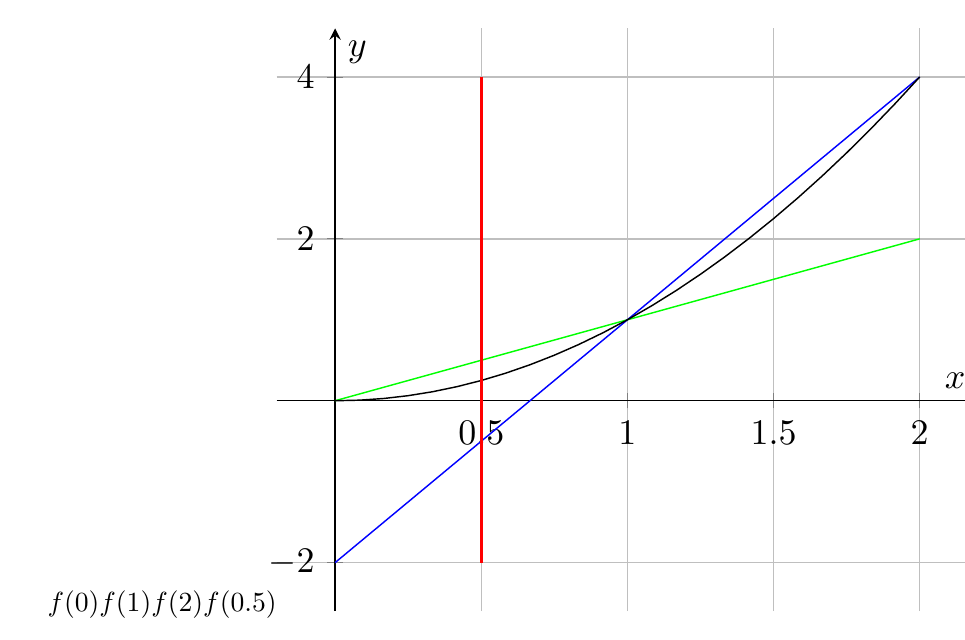
\begin{tikzpicture}[scale=1.3]
				\begin{axis}[
					axis lines=middle,
					xlabel=$x$,
					ylabel=$y$,
					enlargelimits,
					grid=major,
					legend pos=outer north east,
					%ymin=-0.3,
					%xmax=5.8,
					%xticklabels={,,},
					%yticklabels={,,},
					]
					\addplot[color=green, domain=0:2] {x} node[left]{};
					\addplot[color=blue, domain=0:2] {3*x-2} node[left]{};
					\addplot[domain=0:2] {x*x} node[left]{};
					\addplot[color=red, thick] coordinates {
						( 0.5, -2.0 )
						( 0.5, 4 )
					};
					\tikzPoint{60}{$f(0)$}{0,0}
					\tikzPointUp{$f(1)$}{1,1}
					\tikzPointLeft{$f(2)$}{2,4}
					\tikzPointDL{$f(0.5)$}{0.5,0.25}
					\legend{$p_{0,1}$, $p_{1,0}$, $p(x)$}
				\end{axis}
			\end{tikzpicture}
			\caption{Das Ergebnis des Beispiels grafisch. Interpolation erst einmal zwischen jeweils zwei der Punkte ($p[0,1]$ ist hierbei der Punkt bei $x=0.5$ der grünen Linie, $p[1,0]$ die blaue Linie).}
		\end{figure}
	}
	
	\lbreak
	\vertief{
		\n 
		Wenn man in der Aitken-Neville Formel das $x$ einfach als Variable lässt anstelle von einer bestimmten Stelle einzusetzen, wird das Ergebnis äquivalent zu der Interpolationsfunktion von Newton, Lagrange, \dots 
		\n 
		In diesem Fach behandeln wir Aitken-Neville aber so, wie wenn das nicht möglich wäre. Fragt mich nicht warum. \Laughey
	}
	
	\newpage
	\subsubsection{Fehlerabschätzung} \label{sec:interpolation_fehler}
	
	\methode{
		\n
		So kann man den Interpolationsfehler an einer Stelle $x$ abschätzen:
		\begin{align} 
	 		\abs{f(x) - p(x)} = \abs{\frac{f^{(n)}(\xi)}{(n)!} \cdot \prod_{k=0}^{n-1}(x-x_k)} 
	 	\end{align}
		mit $n$ Stützstellen und $\xi$ entspricht einem Wert im Interpolationsbereich (kommt aus dem Mittelwertsatz). Man wählt $\xi$ eigentlich immer so, dass der abgeschätzte Fehler maximal wird. Die Abschätzung des worst-case hat für uns die größte Aussagekraft.
		\n 
		$f^{(n)}$ steht hierbei für die $n$-te Ableitung von $f$.
	}
	

	\sbreak
	\bsp{
		\n
		Wir interpolieren eine Funktion mithilfe von $2$ Stützpunkten an den Stellen $1$ und $4$. Damit ist der Interpolationsbereich definiert mit $x \in [1, 4]$ und wir wollen den Fehler an der Stelle $x = 2$ abschätzen. %In der Aufgabenstellung sei gegeben, dass das größtmögliche $\xi$ gewählt werden soll, also $\xi = 4$.
		\n 
		Wir setzen in obige Formel ein:
		\begin{align*} 
			\abs{f(x) - p(x)} &= \abs{\frac{f^{(2)}(\xi)}{(2)!} \cdot \prod_{k=0}^{2-1}(x-x_k)}  \\
				&= \abs{\frac{f^{(2)}(\xi)}{(2)!} \cdot (2 - x_0)(2 - x_1)}
		\end{align*}
		Sei die zweite Ableitung gegeben, können wir das ganze ausrechnen:
		\begin{align*}
			f"(x) &= \frac{21}{2} \cdot x
		\end{align*}
		Da wir eine worst-case Abschätzung machen wollen, wählen wir $\xi \in [1, 4]$ so, dass die Fehlerabschätzung größtmöglich wird. Hier ist das offensichtlich mit $\xi = 4$ der Fall:
		\begin{align*}
			\abs{f(x) - p(x)} &= \abs{\frac{21 \cdot 4}{2 \cdot 2} \cdot (2 - 1)(2 - 4)}  \\
				&= \abs{21 \cdot 1 \cdot -2} \\
				&= 42
		\end{align*}
		%Da in der zweiten Ableitung kein $x$ mehr vorkommt ist in diesem Fall das $\xi$ völlig irrelevant, da egal wie wir es wählen, das Ergebnis bliebe gleich. \\
		(Dass 42 rauskommt ist kein Zufall \Cooley)
	}

	\newpage
	% =========================================================	
	\subsection{Runge-Effekt}
	% =========================================================
	
	\sbreak
	\defi{
		\n
		Wir haben uns noch nicht mit Problemen der Polynominterpolation beschäftigt. Ein klassisches Beispiel wäre der Runge Effekt.
		\n
		Der Runge Effekt tritt dann auf, wenn man sich mit der Polynominterpolation von Polynomen hohen Grads beschäftigt und äquidistante Stützstellen verwendet. Äquidistant bedeutet hierbei einfach nur, dass diese gleich verteilt sind bzw. der Abstand von jeder Stützstelle zu ihren Nachbarn gleich groß ist. Bisher dachten wir, je mehr Stützstellen wir hinzufügen, desto besser wird auch die Qualität des Interpolationspolynoms.
		\n
		Das ist nicht der Fall. Gerade die Ränder von Interpolationspolynomen mit vielen Stützstellen werden extrem ungenau, das nennen wir den Runge Effekt.
		\n 
		Folgende Erklärung: Wenn wir eine Funktion mit vielen äquidistanten Stützstellen haben, hat unser Interpolationspolynom zwangsläufig einen hohen Grad (ignorieren wir mal triviale Fälle). Wenn dieser hohe Grad informell aber nicht benötigt wird, kommt es zu Schwingungen, speziell an den Rändern des Interpolationsbereiches.
	}

	\picC{runge_pre.png}{0.75}{Interpolation mit wenigen Stützpunkten}
	\picC{runge_solution.png}{0.75}{Dasselbe Problem mit vielen Stützpunkten}
	
	\defi{
		\n 
		Welches der obigen Bilder zeigt die bessere Annäherung der Funktion (gestrichelte Linie) mithilfe von Polynominterpolation (durchgezogene Linie)?
		\n 
		Genau, das obere, welches deutlich weniger Stützpunkte nutzt\dots
	}
